\section{Resultados e discussão}

Nesta sessão serão apresentados e discutidos os resultados provenientes dos ensaios em vazio e com rotor bloqueado do motor de indução cujo circuito equivalente é representado na figura \ref{ckt:1} explicado na metodologia.

Antes de analisar os resultados dos ensaios, faz-se necessário ter conhecimento dos valores de resistência dos enrolamentos do estator que foram medidos, sendo eles:

\begin{table}[H]
\centering
\begin{tabular}{|c|c|}
\cline{1-2}
\textbf{Fase} & \textbf{Resistência ($\Omega$)} \\ \hline
\multicolumn{1}{|c|} u & 6.3 \\ \hline
\multicolumn{1}{|c|} v & 6.3 \\ \hline
\multicolumn{1}{|c|} w & 6.2 \\ \hline
\end{tabular}
\caption{Valores medidos das resistências por enrolamentos do estator.}
\label{tab:1}
\end{table}

Os valores de resistência dos enrolamentos do estator são as únicas grandezas que podem ser medidas diretamente com o multímetro, umas vez que as grandezas do rotor são inacessíveis devido ele estar em gaiola de esquilo e as demais reatâncias serem derivadas da modelagem do circuito equivalente.

\subsection{Ensaio com rotor em vazio}

Com o motor com rotor em vazio, a velocidade do eixo do rotor será bem próxima da velocidade síncrona do campo magnético do estator, assim podendo-se considerar que o escorregamento é aproximadamente nulo ($s \approx 0$). Dessa forma a resistência do rotor tenderá ao infinito ($r_2/s \rightarrow \infty$), evitando que flua corrente para o rotor ($I_2 = 0$), de forma que o circuito equivalente será simplificado para o circuito da figura \ref{ckt:2}.

Como os enrolamentos do estator estavam ligados em estrela (Y), as tensões medidas são as tensões de linha, devendo assim serem transformadas para tensões de fase para a análise do circuito por fase da figura \ref{ckt:2}. Já as correntes de linha são iguais as de fase, assim não necessitando nenhuma transformação. 

Dessa forma, as medições do multimedidor para tensão, corrente e potência, por fase podem ser encontradas na tabela \ref{tab:2}.

\begin{table}[H]
\centering
\begin{tabular}{|c|c|c|c|}
\cline{1-4}
\textbf{Fases} & \textbf{Tensão (V)} & \textbf{Corrente (A)} & \textbf{Potência (W)} \\ \hline
\multicolumn{1}{|c|} u & 218.18 & 1.675 & 40 \\ \hline
\multicolumn{1}{|c|} v & 217.08 & 1.537 & 22 \\ \hline
\multicolumn{1}{|c|} w & 220.83 & 1.549 & 56 \\ \hline
\end{tabular}
\caption{Grandezas do ensaio com rotor em vazio.}
\label{tab:2}
\end{table}

Para encontrar os parâmetros do circuito, inicialmente aplica-se a lei de Ohm da equação \ref{ohm:1} para cada fase com a tensão e corrente medida, assim encontrando a impedância equivalente do circuito equivalente para rotor em vazio, possuindo as parcelas: $r_1$, $x_1$ e $x_{phi}$. 

\begin{equation} \label{ohm:1}
\frac{V_o}{I_o} = \sqrt{r_1^2+(x_1+x_{\phi})^2} 
\end{equation}

Assim os valores conjuntos de $x_1$ e $x_{\phi}$ são encontrados pela equação \ref{res:1} ao serem isolados na equação \ref{ohm:1} para cada uma das fases. 

\begin{equation} \label{res:1}
x_1 + x_{\phi} =  
\left \{
\begin{array}{clcl}
130.10&\Omega, & Fase&u \\
141.09&\Omega, & Fase&v \\
142.43&\Omega, & Fase&w \\
\end{array}
\right.
\end{equation}

Esses resultados podem ser encontrados considerando apenas a partes positiva da resposta, uma vez que não existe reatância negativa. Os valores obtidos em conjunto só podem ser separados após realizar o ensaio de rotor bloqueado.  

Os valores de potência medidos durante o ensaio equivalem a soma das perdas rotacionais com a potência dissipada no resistor $r_1$ do estator. Porém as perdas no estator podem ser calculadas por meio da equação \ref{pot:1}, utilizando a resistência do estator e a corrente de linha medida. Dessa forma as perdas rotacionais podem ser encontradas pela equação \ref{pot:2}.

\begin{equation} \label{pot:1}
P_{estator} = r_1I_{o}^2 = 
\left \{
\begin{array}{clcl}
17.67&W, & Fase&u \\
14.88&W, & Fase&v \\
14.87&W, & Fase&w \\
\end{array}
\right.
\end{equation}

\begin{equation} \label{pot:2}
P_{rotacionais} = P_{o} - P_{estator} =  
\left \{
\begin{array}{clcl}
22.32&W, & Fase&u \\
7.11&W, & Fase&v \\
41.12&W, & Fase&w \\
\end{array}
\right.
\end{equation}

\subsection{Ensaio com rotor bloqueado}

Com o motor com o rotor bloqueado, a velocidade do eixo do rotor será nula, permitindo que o escorregamento seja unitário ($s=1$). Isso reflete na resistência do rotor de forma a deixar o valor puro da resistência ($r_2/s = r_2$), permitindo encontrar seu valor. Outra consideração é que, como os valores de $r_2$ e $x_2$ são bem menores que $x_{\phi}$, a corrente que irá para este é desprezível à corrente que irá para os demais, podendo assim desconsiderar essa reatância do circuito equivalente, resultando no circuito da figura \ref{ckt:3} a ser analisado no ensaio com rotor bloqueado.

Da mesma forma que o ensaio anterior, os enrolamentos do estator estavam ligados em estrela (Y), fazendo assim as mesmas considerações para as tensões e correntes.

Dessa forma, as medições do multimedidor para tensão, corrente e potência, por fase podem ser encontradas na tabela \ref{tab:3}.

\begin{table}[H]
\centering
\begin{tabular}{|c|c|c|c|}
\cline{1-4}
\textbf{Fases} & \textbf{Tensão (V)} & \textbf{Corrente (A)} & \textbf{Potência (W)} \\ \hline
\multicolumn{1}{|c|} u & 37.23 & 2.541 & 65  \\ \hline
\multicolumn{1}{|c|} v & 37.06 & 2.513 & 64 \\ \hline
\multicolumn{1}{|c|} w & 37.58 & 2.498 & 65 \\ \hline
\end{tabular}
\caption{Grandezas do ensaio com rotor bloqueado.}
\label{tab:3}
\end{table}

Por meio da análise do circuito equivalente da figura \ref{ckt:3}, observa-se que a potência medida equivale às perdas nas resistências do estator ($r_1$) e do rotor ($r_2$). Nesse caso não há perdas rotacionais, uma vez que o rotor está bloqueado. Dessa forma as perdas podem ser equacionadas pela equação \ref{pot:3} e permitindo isolar $r_2$ encontrar o seu valor por fase na equação \ref{pot:4}, uma vez que $r_1$ já é conhecido.

\begin{equation} \label{pot:3}
P_{rb} = (r_1+r_2)I_{rb}^2 
\end{equation}

\begin{equation} \label{pot:4}
r_2 = \frac{P_{rb}}{I_{rb}^2}-r_1 =  
\left \{
\begin{array}{clcl}
3.76&\Omega, & Fase&u \\
3.83&\Omega, & Fase&v \\
4.21&\Omega, & Fase&w \\
\end{array}
\right.
\end{equation}

Para encontrar os parâmetros restantes, faz-se novamente a lei de Ohm com a tensão e correntes medidas para cada fase para encontrar a impedância equivalente do circuito equivalente para o rotor bloqueado, de forma a obedecer a equação \ref{ohm:2}, possuindo as parcelas: $r_1$, $r_2$, $x_1$ e $x_2$.

\begin{equation} \label{ohm:2}
\frac{V_{rb}}{I_{rb}} = \sqrt{(r_1+r_2)^2+(x_1+x_2)^2} 
\end{equation}

Assim os valores conjuntos de $x_1$ e $x_2$ são encontrados pela equação \ref{res:2} ao serem isolados na equação \ref{ohm:2} para cada uma das fases e substituindo os valores de tensão, corrente, $r_1$ e $r_2$. 

\begin{equation} \label{res:2}
x_1 + x_2 =  
\left \{
\begin{array}{clcl}
10.65&\Omega, & Fase&u \\
10.71&\Omega, & Fase&v \\
10.85&\Omega, & Fase&w \\
\end{array}
\right.
\end{equation}

Para título de simplificação, considera-se que as reatâncias série do estator e do rotor são iguais ($x_1=x_2$). Assim, obtém-se seus valores individuais em \ref{res:3}

\begin{equation} \label{res:3}
x_1 = x_2 =  
\left \{
\begin{array}{clcl}
5.32&\Omega, & Fase&u \\
5.35&\Omega, & Fase&v \\
5.42&\Omega, & Fase&w \\
\end{array}
\right.
\end{equation}

Por fim, com os valores de $x_1+x_{\phi}$ encontrados no ensaio anterior, agora se torna possível separar essa soma, uma vez que os valores de $x_1$ foram encontrados, de forma que os valores de $x_{\phi}$ podem ser observados na equação \ref{res:4}.

\begin{equation} \label{res:4}
x_{\phi} =  
\left \{
\begin{array}{clcl}
124.77&\Omega, & Fase&u \\
135.73&\Omega, & Fase&v \\
137.00&\Omega, & Fase&w \\
\end{array}
\right.
\end{equation}

\subsection{Circuito equivalente com os parâmetros definidos}

Com todos os parâmetros do circuito equivalente encontrados, pode-se observar seus valores aplicados no circuito equivalente para a fase u na figura \ref{ckt:5}. Para os circuitos equivalentes das demais fase o raciocínio é o mesmo.


\begin{figure}[H]
\begin{center}
\tikz  {
\begin{tikzpicture} [ american, ]
    \draw (0,0) -- (8.5,0)
    (0,3) to[R, f_>=$I_1$, l=$6.3 \Omega$] (3,3)
    (3,3) to[L, l=$5.32 \Omega$] (6,3)
    (6,3) to[L, f_>=$I_2$, l=$5.32 \Omega$] (9,3) -- (9.5,3)
    (6,3) to[L, f=$I_{\phi}$, l=$124.77 \Omega$] (6,0)
    (9.5,3) -- (9.5,2.5) 
    (9.5,1) to[pR, l_=$\frac{3.76}{s} \Omega$] (9.5,2.5) 
    (9,1.75) -- (8.5,1.75) -- (8.5,0)
    (0,1.5) node{$V_1$}
    ;
\end{tikzpicture}
}
\end{center}
\caption{Circuito equivalente para o motor de indução com os valores calculados para a fase u.}
\label{ckt:5} 
\end{figure}

\subsection{Curva de torque-escorregamento}

Para traçar a curva de torque-escorregamento, inicialmente calcula-se os parâmetros do circuito equivalente de Thévenin a título de simplificação dos cálculos. Os parâmetros a serem obtidos obedecem o formado do circuito da figura \ref{ckt:4}.

Onde a impedância equivalente de Thévenin é calculada a partir do circuito da figura \ref{ckt:1} por meio da equação \ref{the:1} e a tensão de Thévenin é calculada por meio da equação \ref{the:2}

\begin{equation} \label{the:1}
R_1 + jX_1 = (r_1+jx_1) || jx_{\phi}  
\end{equation}

\begin{equation} \label{the:2}
V_{TH} = V_1\frac{jx_{\phi}}{(r_1+jx_1)+jx_{\phi}}  
\end{equation}

Substituindo os valores, encontram-se as respostas por fase nas equações \ref{the:3} e \ref{the:4}.

\begin{equation} \label{the:3}
R_1+jX_1 =  
\left \{
\begin{array}{clcl}
5.78+j5.38&\Omega, & Fase&u \\
5.81+j5.41&\Omega, & Fase&v \\
5.72+j5.47&\Omega, & Fase&w \\
\end{array}
\right.
\end{equation}

\begin{equation} \label{the:4}
V_{TH}=  
\left \{
\begin{array}{clcl}
208.76+j10.10&V, & Fase&u \\
208.42+j9.30&V, & Fase&v \\
212.01+j9.22&V, & Fase&w \\
\end{array}
\right.
\end{equation}

Esses valores no circuito equivalente de Thévenin para a fase u podem ser encontrados no circuito da figura \ref{ckt:6}. O raciocínio é semelhante para as demais fases.


\begin{figure}[H]
\begin{center}
\tikz  {
\begin{tikzpicture} [ american, ]
    \draw (0,0) -- (8.5,0)
    (0,3) to[R, f_>=$I_2$, l=$5.78\Omega$] (3,3)
    (3,3) to[L, l=$j5.38\Omega$] (6,3)
    (6,3) to[L, l=$j5.32\Omega$] (9,3) -- (9.5,3)
    (9.5,3) -- (9.5,2.5) 
    (9.5,1) to[pR, l_=$\frac{3.76}{s}\Omega$] (9.5,2.5) 
    (9,1.75) -- (8.5,1.75) -- (8.5,0)
    (0,1.5) node{$209\angle2.77^{\circ}V$}
    ;
\end{tikzpicture}
}
\end{center}
\caption{Circuito equivalente de Thévenin para o motor de indução com os valores calculados para a fase u.}
\label{ckt:6} 
\end{figure}


A curva de conjugado e escorregamento vai obedecer a equação \ref{ts:1} (FITZGERALD, 2014).

\begin{equation} \label{ts:1}
T=\frac{1}{\omega_s}\frac{V_{TH}^2q_1\frac{r_2}{s}}{\left(R_1+\frac{r_2}{s}\right)^2+(X_1+x_2)^2}
\end{equation}

Onde:
\begin{itemize}
    \item $\omega_s$ é a velocidade angular síncrona;
    \item $q_1$ é o número de fases (no caso são 3 fases);
    \item $s$ é o escorregamento ($s=\frac{n_s-n}{n_s}$, com $n_s$ a velocidade síncrona e $n$ a velocidade do eixo do rotor, ambas em RPM).
\end{itemize}
\pagebreak

Porém como não se dispõe da velocidade angular síncrona ($\omega_s$), se faz necessário consultar na placa do motor na figura \ref{placa} os valores da potência e velocidade em plena carga do eixo do rotor. Dessa forma, obtém-se os seguintes valores:

\begin{center}
    $P_{eixo_N} = 1100 W$ \vspace{5pt}\\
    $n_{eixo_N} = 1715 RPM$
\end{center}

Assim, também se conclui que a máquina possui 4 polos ($N_p = 4$), ao considerar que a velocidade síncrona mais próxima da velocidade do eixo é 1800 RPM ($n_{estator}=1800 RPM$) para a frequência de 60 Hz ($f=60Hz$) da rede de alimentação do estator.

Considerando que as perdas rotacionais se mantém constantes e adotando a análise unicamente para a fase u, obtém-se a potência mecânica interna nominal ($P_{mec_N}$) por meio da equação \ref{conj:1}.

\begin{equation} \label{conj:1}
P_{mec_N} = P_{eixo_N} + P_{rotacionais} = 1100 + 22.32 = 1122.32 W
\end{equation}

Pela relação de transformação de rad/s para RPM, a velocidade nominal do eixo do motor pode ser escrita de acordo com a equação \ref{conj:2}].

\begin{equation} \label{conj:2}
\omega_{eixo_N} = n_{eixo_N}\times \frac{2\pi}{60} = 179.6 rad/s
\end{equation}

Outras relações conhecidas e que podem ser utilizadas para determinar a velocidade síncrona é a relação que o conjugado nominal pode ser encontrado como uma relação entre a potência nominal do entreferro com a velocidade síncrona pela equação \ref{conj:3}. Porém a velocidade síncrona pode ser escrita em função da velocidade do eixo encontrada na placa da máquina com o complementar do escorregamento nominal da máquina na equação \ref{conj:4}. A potência do nominal do entreferro também pode ser escrita em função da potência mecânica interna nominal e do complemento do escorregamento nominal na equação \ref{conj:5}.

\begin{equation} \label{conj:3}
T_N = \frac{P_{gN}}{\omega_s}
\end{equation}

\begin{equation} \label{conj:4}
\omega_s= \frac{\omega_{eixo_N}}{1-s_N}
\end{equation}

\begin{equation} \label{conj:5}
P_{gN} = \frac{P_{mec_N}}{1-s_N}
\end{equation}

Substituindo as equações \ref{conj:4} e \ref{conj:5} em \ref{conj:3}, obtém-se o torque nominal na equação \ref{conj:6}, independente do valor do escorregamento.

\begin{equation} \label{conj:6}
T_N = \frac{P_{mec_N}}{1-s_N}\times\frac{1-s_N}{\omega_{eixo_N}} = 9.12 Nm
\end{equation}

Conhecendo o valor do conjugado nominal, se torna possível calcular o valor do escorregamento nominal ($s_N$) por meio da substituição da equação \ref{conj:4} na equação do conjugado em \ref{ts:1}, obtendo assim a equação \ref{conj:7}.

\begin{equation} \label{conj:7}
T=\frac{1-s_N}{\omega_{eixo_N}}\frac{V_{TH}^2q_1\frac{r_2}{s}}{\left(R_1+\frac{r_2}{s}\right)^2+(X_1+x_2)^2} = 9.12
\end{equation}

Para solucionar a equação \ref{conj:7} para encontrar os valores de escorregamento foi utilizada a função \textbf{fsolve()} do Scilab, da forma como foi implementada no script no apêndice desse trabalho, permitindo encontrar três valores possível de escorregamento nominal para cada uma das fases. Para a fase u foram obtidos os seguintes valores:

\begin{center}
    $s_{N1} = 0$ \vspace{5pt}\\
    $s_{N2} = 0.0379$ \vspace{5pt}\\
    $s_{N3} = 0.636$
\end{center}

A resposta oferecida $s_{N1}$ não é útil, pois é conhecido que o escorregamento é próximo à zero apenas com o rotor em vazio. Para se ter conhecimento da resposta correta, deve-se calcular o escorregamento máximo a partir da equação \ref{conj:8}. Isso, pois em plena carga o escorregamento é normalmente menor que o que o escorregamento de conjugado máximo.

\begin{equation} \label{conj:8}
s_{max} = \frac{r_2}{\sqrt{R_{1}^2+(X_1+x_2)^2}} = 0.309
\end{equation}

Dessa forma o valor de $s_{N3}$ é descartado, restanto que o escorregamento nominal é o valor de $s_{N2}$, de cerca de 3.79\%.

Assim, aplicando o valor de escorregamento nominal encontrado à equação \ref{conj:4} pode-se encontrar a velocidade síncrona e aplicar à equação \ref{ts:1} para encontrar a expressão do conjugado em função do escorregamento na equação para a fase u \ref{ts:2}. Para as demais fases o raciocínio é o mesmo trabalho nessa sessão.

\begin{equation} \label{conj:9}
\omega_s= \frac{\omega_{eixo_N}}{1-s_N} = \frac{179.6}{1-0.0379} = 186.67 rad/s
\end{equation}

\begin{equation} \label{ts:2}
T=\frac{1}{186.67}\frac{(209)^2\times3\times\frac{3.76}{s}}{\left(5.78+\frac{3.76}{s}\right)^2+(5.38+5.32)^2} 
\end{equation}

Assim, ao simular a curva de conjugado e escorregamento no Scilab para as três fases, obtém-se a figura \ref{curv:1}. 

\begin{figure}[H]
\centering
    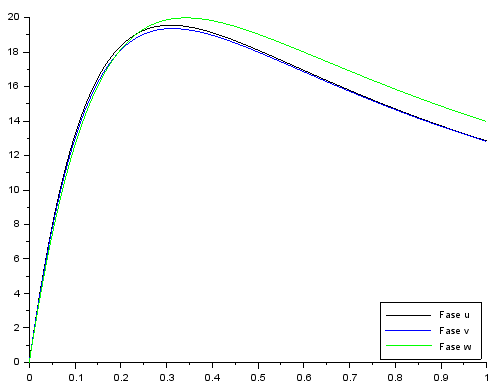
\includegraphics[width=10cm]{images/ts1.png}  
\caption{Curvas de conjugado e escorregamento para cada uma das fases do motor.}
\label{curv:1} 
\end{figure}

Avaliando os vetores obtidos na simulação, observa-se que o conjugado máximo foi obtido nos pontos onde o escorregamento é máximo, gerando assim a tabela \ref{results:1}. Já para o conjugado de partida, o ponto em que estes podem ser encontrados é quando o valor do escorregamento for unitário, gerando assim a tabela \ref{results:2} com os respectivos dados.

\begin{table}[H]
\centering
\begin{tabular}{|c|c|c|}
\cline{1-3}
\textbf{Fases} & \textbf{Conjugado (Nm)} & \textbf{Escorregamento} \\ \hline
\multicolumn{1}{|c|} u & 19.55 & 0.309 \\ \hline
\multicolumn{1}{|c|} v & 19.35 & 0.313 \\ \hline
\multicolumn{1}{|c|} w & 19.97 & 0.342 \\ \hline
\end{tabular}
\caption{Valores de conjugado máximo e os respectivos valores de escorregamento para cada fase.}
\label{results:1}
\end{table}

\begin{table}[H]
\centering
\begin{tabular}{|c|c|c|}
\cline{1-3}
\textbf{Fases} & \textbf{Conjugado (Nm)} & \textbf{Escorregamento} \\ \hline
\multicolumn{1}{|c|} u & 12.84 & 1 \\ \hline
\multicolumn{1}{|c|} v & 12.81 & 1 \\ \hline
\multicolumn{1}{|c|} w & 13.96 & 1 \\ \hline
\end{tabular}
\caption{Valores de conjugado de partida para cada fase.}
\label{results:2}
\end{table}

Assim observa-se que o conjugado de partida é bem menor que o conjugado máximo, porém ainda são maiores do que os valores de operação nominal.

\subsection{Conjugado máximo na partida}

Supondo que o motor ensaiado é de rotor bobinado, ou seja, há a possibilidade de acesso aos enrolamentos do motor, propõe-se descobrir qual resistência que associada em série e por fase ao circuito do rotor resulte em um conjugado máximo na partida.

Assim, considera-se a equação \ref{max:1} para calcular o valor da nova resistência $r_{2}^{'}$ do rotor, de forma que ela é composta pela soma da antiga parcela e da nova parcela a ser associada em série para obter o conjugado máximo na partida de forma que: $r_{2}^{'} = r_2 + r_{adicional}$. Vale destacar que o escorregamento máximo é igualado ao escorregamento unitário de partida.

\begin{equation} \label{max:1}
s_{max} = \frac{r_2}{\sqrt{R_{1}^2+(X_1+x_2)^2}} = 1
\end{equation}

\begin{equation} \label{max:2}
r_{adicional} = \sqrt{R_{1}^2+(X_1+x_2)^2} - r_2
\end{equation}

Assim, permite-se isolar o valor de resistência a ser associado e calcular o seu valor, tendo como base os valores encontrados em ensaios anteriores, obtendo-se os valores por fase da resistência adicional na tabela \ref{results:3}.

\begin{table}[H]
\centering
\begin{tabular}{|c|c|}
\cline{1-2}
\textbf{Fases} & Resistência adicional ($\Omega$)  \\ \hline
\multicolumn{1}{|c|} u & 8.40  \\ \hline
\multicolumn{1}{|c|} v & 8.40  \\ \hline
\multicolumn{1}{|c|} w & 8.09  \\ \hline
\end{tabular}
\caption{Valores de resistência adicional par ao rotor bobinado para cada fase.}
\label{results:3}
\end{table}

Portanto, mais uma vez pode-se traçar a curva de conjugado e escorregamento na figura \ref{curv:2} observando que os valores de torque máximo são obtidos na partida.

\begin{figure}[H]
\centering
    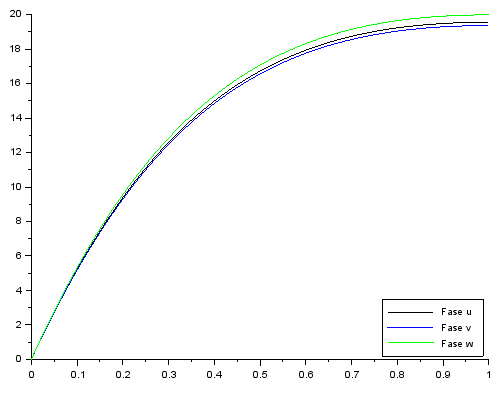
\includegraphics[width=10cm]{images/ts2.png}  
\caption{Curvas de conjugado e escorregamento para cada uma das fases do motor para uma dada resistência em série com o enrolamentos do rotor que resulta no conjugado máximo na partida.}
\label{curv:2} 
\end{figure}

Porém para a máquina que foi ensaiada isso é impossível, pois seu rotor é disposto na forma de gaiola de esquilo, não havendo acesso aos seus enrolamentos, uma vez que são curto-circuitados.